%                                                                 aa.dem
% AA vers. 9.0, LaTeX class for Astronomy & Astrophysics
% demonstration file
%                                                       (c) EDP Sciences
%-----------------------------------------------------------------------
%
%\documentclass[referee]{aa} % for a referee version
%\documentclass[onecolumn]{aa} % for a paper on 1 column  
%\documentclass[longauth]{aa} % for the long lists of affiliations 
%\documentclass[rnote]{aa} % for the research notes
%\documentclass[letter]{aa} % for the letters 
%\documentclass[bibyear]{aa} % if the references are not structured 
%                              according to the author-year natbib style

% \documentclass[]{aa}  
\documentclass[traditabstract]{aa}  

\usepackage{graphicx}
\usepackage{txfonts}
\usepackage{url}
% The [draft] was added to avoid a LaTeX issue
% See https://tex.stackexchange.com/a/154184
\usepackage[draft]{hyperref}

\begin{document} 

\newcommand{\PythonUrl}{\url{http://fits.gsfc.nasa.gov/}\xspace}
\newcommand{\FitsUrl}{\url{http://fits.gsfc.nasa.gov/}\xspace}
\newcommand{\GammapyUrl}{\url{http://gammapy.org}\xspace}
\newcommand{\GadfUrl}{\url{http://gamma-astro-data-formats.readthedocs.io/}\xspace}
\newcommand{\ReadthedocsUrl}{\url{https://readthedocs.org/}\xspace}
\newcommand{\TravisUrl}{\url{https://www.travis-ci.org/}\xspace}

\newcommand{\NaimaUrl}{\url{https://github.com/zblz/naima}\xspace}


% Note: not sure if we want to use that ... doesn't look too pretty
% \newcommand{\astropy}{\texttt{Astropy}\xspace}
% \newcommand{\gammapy}{\texttt{Gammapy}\xspace}


% Front matter
\title{Gammapy: A Python package for gamma-ray astronomy}
\titlerunning{Gammapy}
\authorrunning{Deil, Donath, Terrier et al.}

\author{
Gammapy contributors (author list tbd)
% Christoph Deil\inst{\ref{inst:mpik}}
% \and
% Axel Donath\inst{\ref{inst:mpik}}
% \and
% Régis Terrier\inst{\ref{inst:apc}}
% \and
% Johannes King\inst{\ref{inst:mpik}}
% \and
% Léa Jouvin\inst{\ref{inst:apc}}
% \and
% Manuel Paz Arribas\inst{\ref{inst:humboldt}}
% \and
% Ellis Owen\inst{\ref{inst:ucl}}
% \and
% Julien Lefaucheur\inst{\ref{inst:obsparis}}
% \and
% Olga Vorokh\inst{\ref{inst:olga}}
% \and
% Jonathan Harris\inst{\ref{inst:jon}}
% \and
% Brigitta Sipocz\inst{\ref{inst:brigitta1}, \ref{inst:brigitta2}}
% \and
% Dirk Lennarz\inst{\ref{inst:atlanta}}
% \and
% Helen Poon\inst{\ref{inst:mpik}}
% \and
% Nachiketa Chakraborty\inst{\ref{inst:mpik}}
% \and
% Domenico Tiziani\inst{\ref{inst:erlangen}}
% \and
% Luigi Tibaldo\inst{\ref{inst:mpik}}
% \and
% Victor Zabalza\inst{\ref{inst:victor}}
% \and
% Rolf Bühler\inst{\ref{inst:desy}}
% \and
% Stefan Klepser\inst{\ref{inst:desy}}
% \and
% Ignasi Reichardt\inst{\ref{inst:padova}}
}

\institute{
% Max-Planck-Institut f\"{u}r Kernphysik, Heidelberg, Germany
% \label{inst:mpik}
% \and
% APC, University of Paris 7, France
% \label{inst:apc}
% \and
% LUTH, Observatoire de Paris, Meudon, France
% \label{inst:obsparis}
% \and
% DESY, Zeuthen, Germany
% \label{inst:desy}
% \and
% Humboldt University, Berlin, Germany
% \label{inst:humboldt}
% \and
% UCL-MSSL, Dorking, United Kingdom
% \label{inst:ucl}
% \and
% INFN, Padova, Italy
% \label{inst:padova}
% \and
% Belarusian State University, Belarus, Minsk
% \label{inst:olga}
% \and
% FAU, Erlangen, Germany
% \label{inst:erlangen}
% \and
% School of Physics and Center for Relativistic Astrophysics, Georgia
% Institute of Technology, Atlanta, GA, USA
% \label{inst:atlanta}
% \and
% Centre for Astrophysics Research, University of Hertfordshire, College Lane, Hatfield, AL10 9AB, UK
% \label{inst:brigitta1}
% \and
% Institute of Astronomy, University of Cambridge, Madingley Road, Cambridge, CB3 0HA, UK
% \label{inst:brigitta2}
% \and
% Department of Physics, Durham University, South Road, Durham, DH1 3LE, UK
% \label{inst:jon}
% \and
% TODO: Victor address
% \label{inst:victor}
}

% \abstract{}{}{}{}{} 
% 5 {} token are mandatory

\abstract{

We present the first major version v1.0 of the open-source and community developed
software package \gammapy.

% context heading (optional)
% {} leave it empty if necessary  
{Gammapy context: HESS, CTA, Fermi, open data, open-source, Python, community}

% aims heading (mandatory)
{Gammapy aims}

% methods heading (mandatory)
{Gammapy methods}

% results heading (mandatory)
{Gammapy results}

% conclusions heading (optional), leave it empty if necessary 
{Gammapy conclusions}
}

% \date{Received September 15, 1996; accepted March 16, 1997}
\keywords{
Gamma rays: general - 
Astronomical instrumentation, methods and techniques - 
Methods: data analysis
}

\maketitle

% Main part
\section{Introduction}
\label{sec:intro}
Gamma-ray astronomy is a rather young field of research.
By detecting and reconstructing arrival direction, time and energy
of primary cosmic gamma-rays
The gamma-ray sky is either observed by ground based instruments

, driven by experiments with proprietary software often based
on ROOT, because of the particle physics background. Such 
as HESS, Veritas or Magic.

The Cherenkov Telescope Array will be operated as an open
observatory for the first time. Thus there is a need for
open analysis software as well.

Once the primary photons are reconstructed the format of the data
of all Gamma-ray instrumets can be brought into a common format.
An effort is the gamma-astro data formats \cite{gadf-zenodo}.
The data format is based on FITS  \citep{fits}.


In recent years Python \footnote{\PythonUrl} has established as one of the
standard programming  languages for astronomy \footnote{Citation missing}
as well as data sciences in  general \footnote{Citation missing}.
The success is mostly attributed to the simple and easy to learn syntax,
the ability to act as a "glue" language between different libraries,
the rich eco-system of packages and the open and active (online) community.

Astronomical data analysis software written in Python existed since 2000.
e.g. sherpa \citep{sherpa-2011, sherpa-2009}, or for gamma-ray even
PyFACT \citep{pyfact}.

The short-term success of Pythion lead to a prolifaration of packages, until
\astropy \citep{astropy} was created in 2012. Astropy is and


Gammapy is a Python package for gamma-ray astronomy.

% TODO: describe Context

% TODO: describe goals

TODO: Figure 1: Data -> Gammapy -> Spectra etc with some details 

Basic idea: build on Numpy and Astropy, use Python stack

TODO: Figure 2: Gammapy software stack

Here's a list of references I'd like to cite ... to be incorporated into the
main text somewhere:

\begin{itemize}
\item Gammapy webpage\footnote{\GammapyUrl}
\item Naima\footnote{\NaimaUrl} \citep{Naima}
\item Gammapy use in science publications: \citep{Owen2015}, SNR shell, HGPS
\end{itemize}

* Gammapy – A Python package for gamma-ray astronomy
* Gammapy – A prototype for the CTA science tools 
* Astropy: A community Python package for astronomy
* THE ASTROPY PROJECT: BUILDING AN INCLUSIVE, OPEN-SCIENCE PROJECT AND STATUS OF THE V2.0 CORE PACKAGE
* GammaLib and ctools
* Fermipy proceedings
* SunPy: Python for Solar Physics. An implementation for local correlation tracking
*

\begin{figure}[t]
\centering
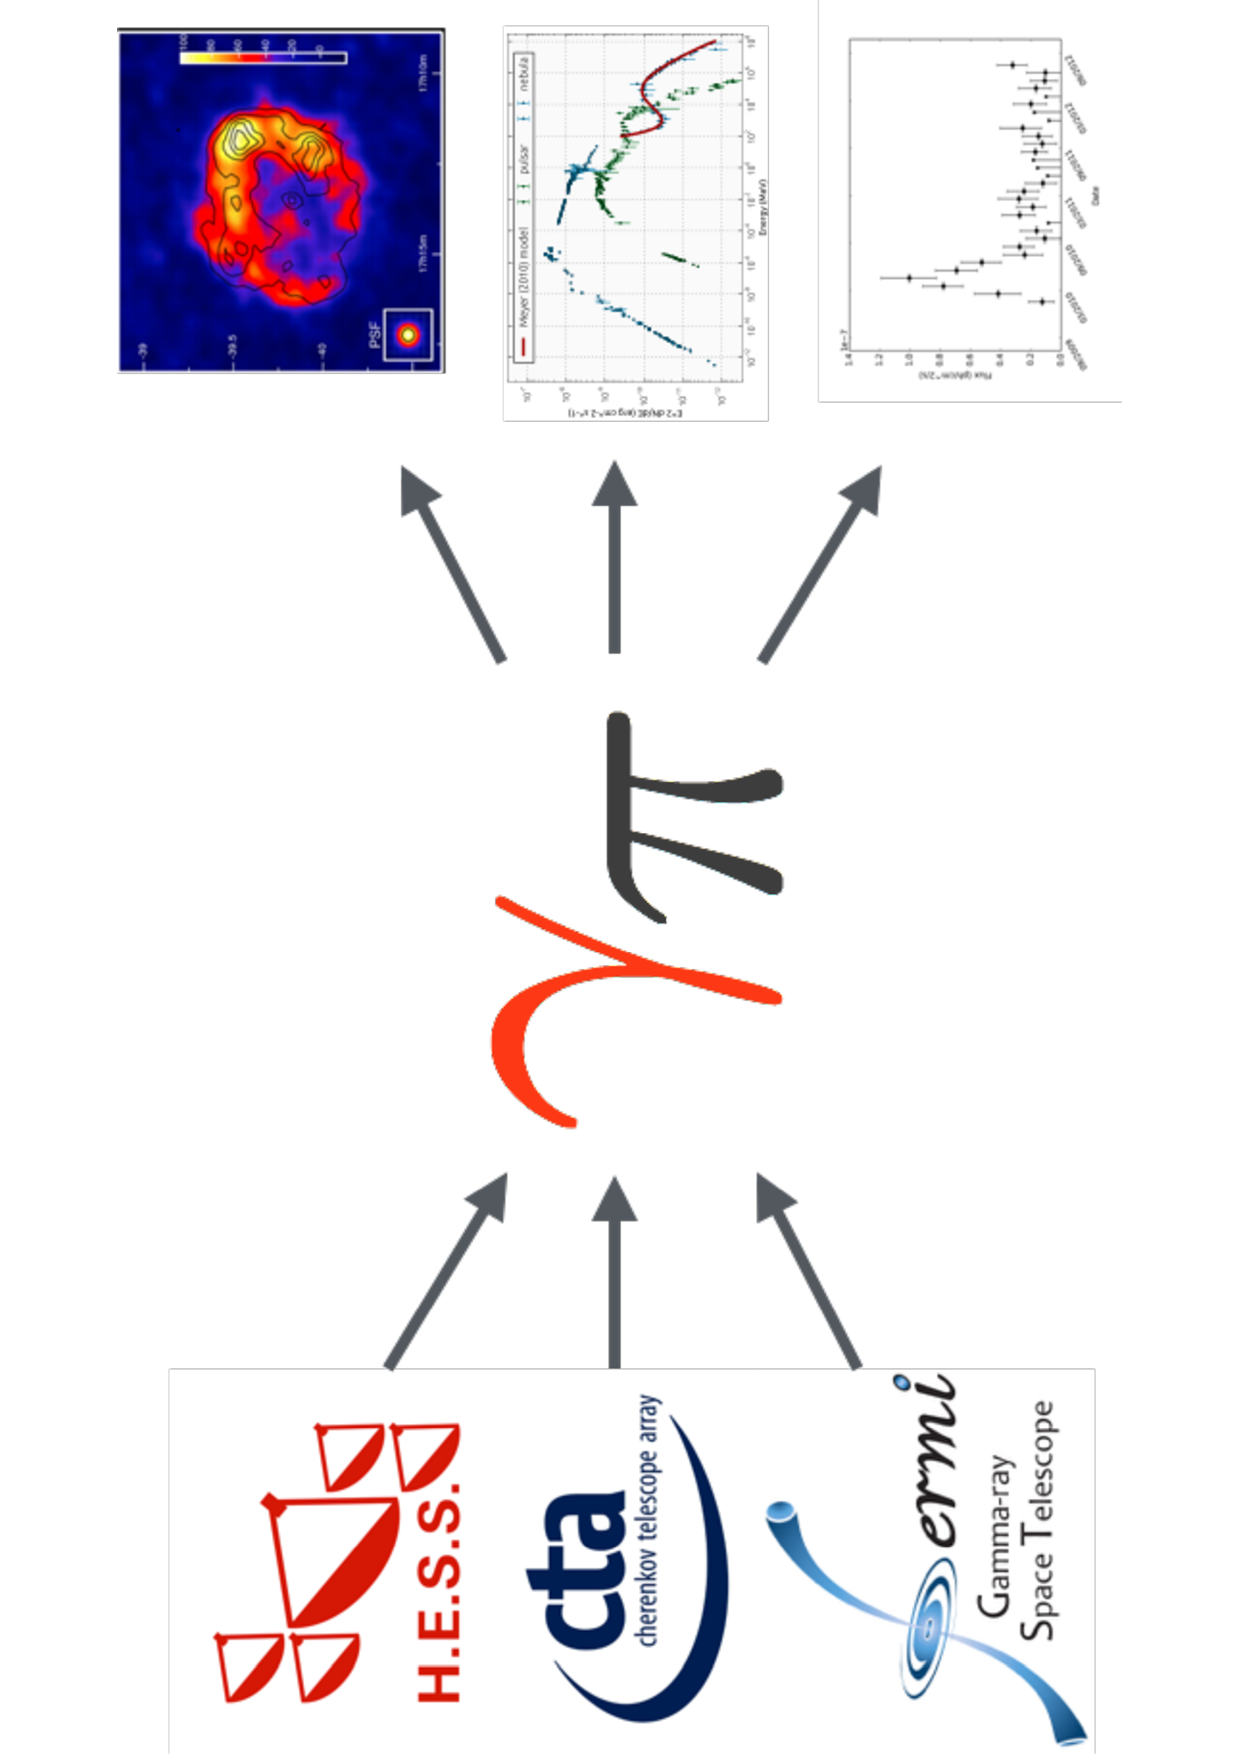
\includegraphics[height=0.5\textwidth, angle=270]{figures/gammapy-big-picture}
\caption{
Gammapy is a Python package for high-level gamma-ray data analysis. Using event
lists, exposures and point spread functions as input you can use it to generate
science results such as images, spectra, light curves or source catalogs. So far
it has been used to simulate and analyse H.E.S.S., CTA and \textit{Fermi}-LAT
data, hopefully it will also be applied to e.g. VERITAS, MAGIC or HAWC data in
the future.
}
\label{fig:big-picture}
\end{figure}

\begin{figure}[t]
\centering
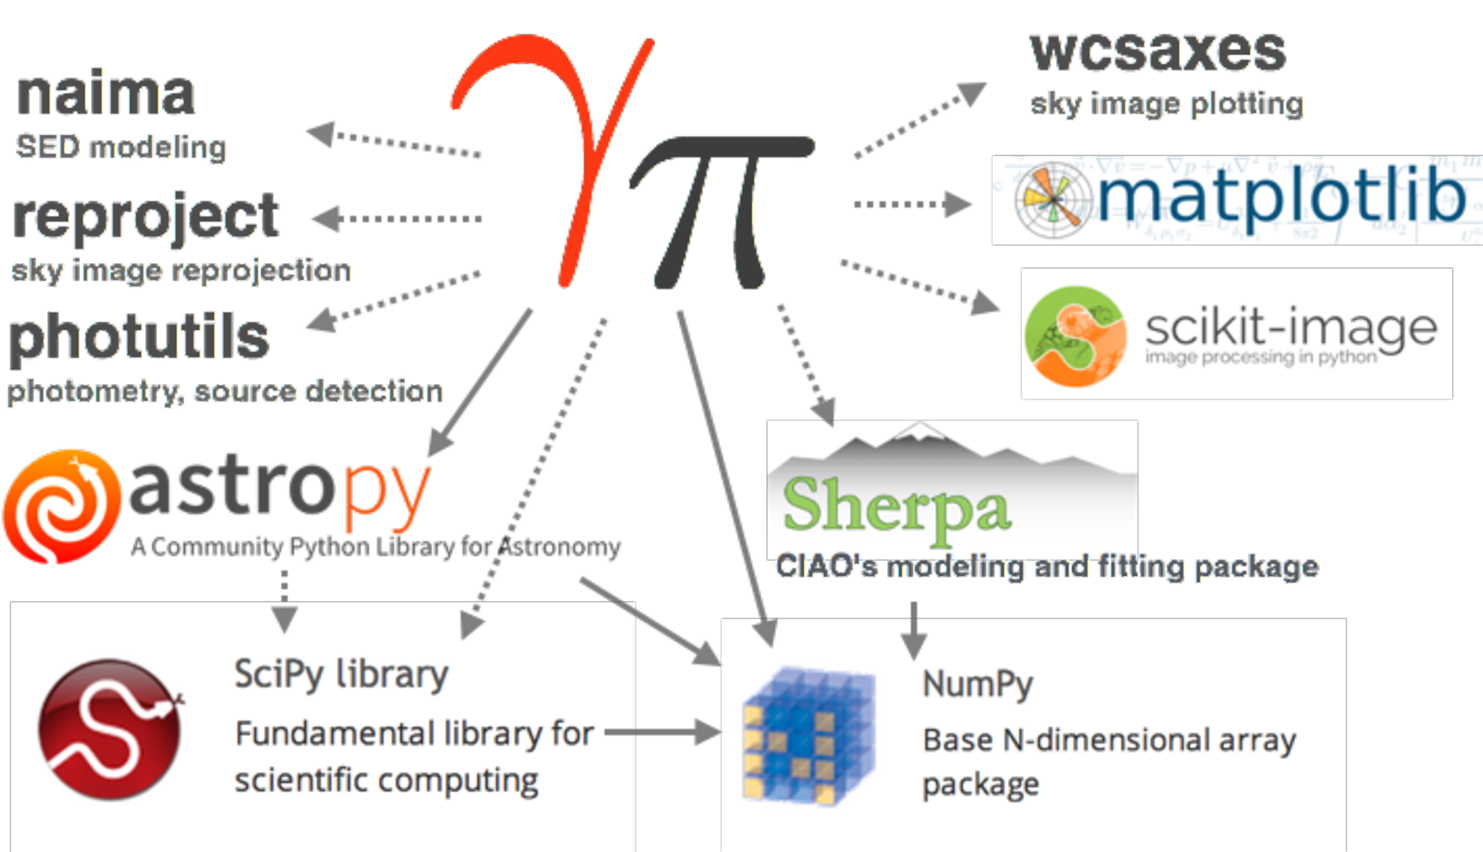
\includegraphics[width=0.5\textwidth]{figures/gammapy-dependencies}
\caption{
The Gammapy stack. Required dependencies Numpy and Astropy are illustrated with
solid arrows, optional dependencies (the rest) with dashed arrows.
}
\label{fig:dependencies}
\end{figure}

\section{Gammapy package}
\label{sec:package}

Outline:
* List typical analysis use cases
* Can use from Python and Jupyter -> show Figure with Jupyter notebook here.
* Gammapy code structure
* How Numpy and Astropy is used


Figures:
* Add a Figure showing dataflow in a typical application
DL3 at the top, spectrum, map, lightcurve, fit results at the bottom.
Mention major classes in between (DataStore, EventList, Map, MapMaker, MapFit, …)
* Probably not: Figure showing sub-packages and how they relate (gammapy.data and gammapy.irf at the base, then gammapy.maps, etc.
* The code example Figure how to make a counts map, to explain how the package works.

\section{Applications}
\label{sec:apps}

Each application example is a notebook in the online material: We could have one
analysis as Python scripts instead of notebook in the online material. At the
start of this section, point to gammapy-paper repo on Github and say that
there’s a Binder where people can try the examples online.

TODO: mention other application examples (joint Crab paper, HESS validation
paper, HGPS, ...) here or in a subsection "other applications" at the end of
this section?

\subsection{Source detection}
\label{apps:detect}

See Figure~\ref{fig:fermi-ts-image}.

Ref: \citep{Stewart2009}

\begin{figure*}[t]
\centering
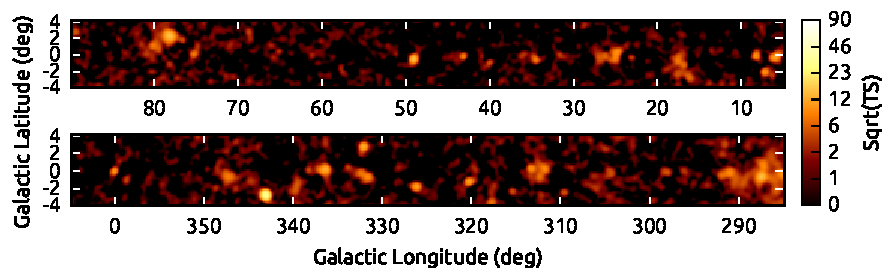
\includegraphics[width=1.\textwidth]{figures/gammapy-fermi-ts-image}
\caption{
Gammapy application example: A \textit{Fermi} survey TS map of the inner
Galactic plane region.
}
\label{fig:fermi-ts-image}
\end{figure*}

\begin{figure*}[t]
\centering
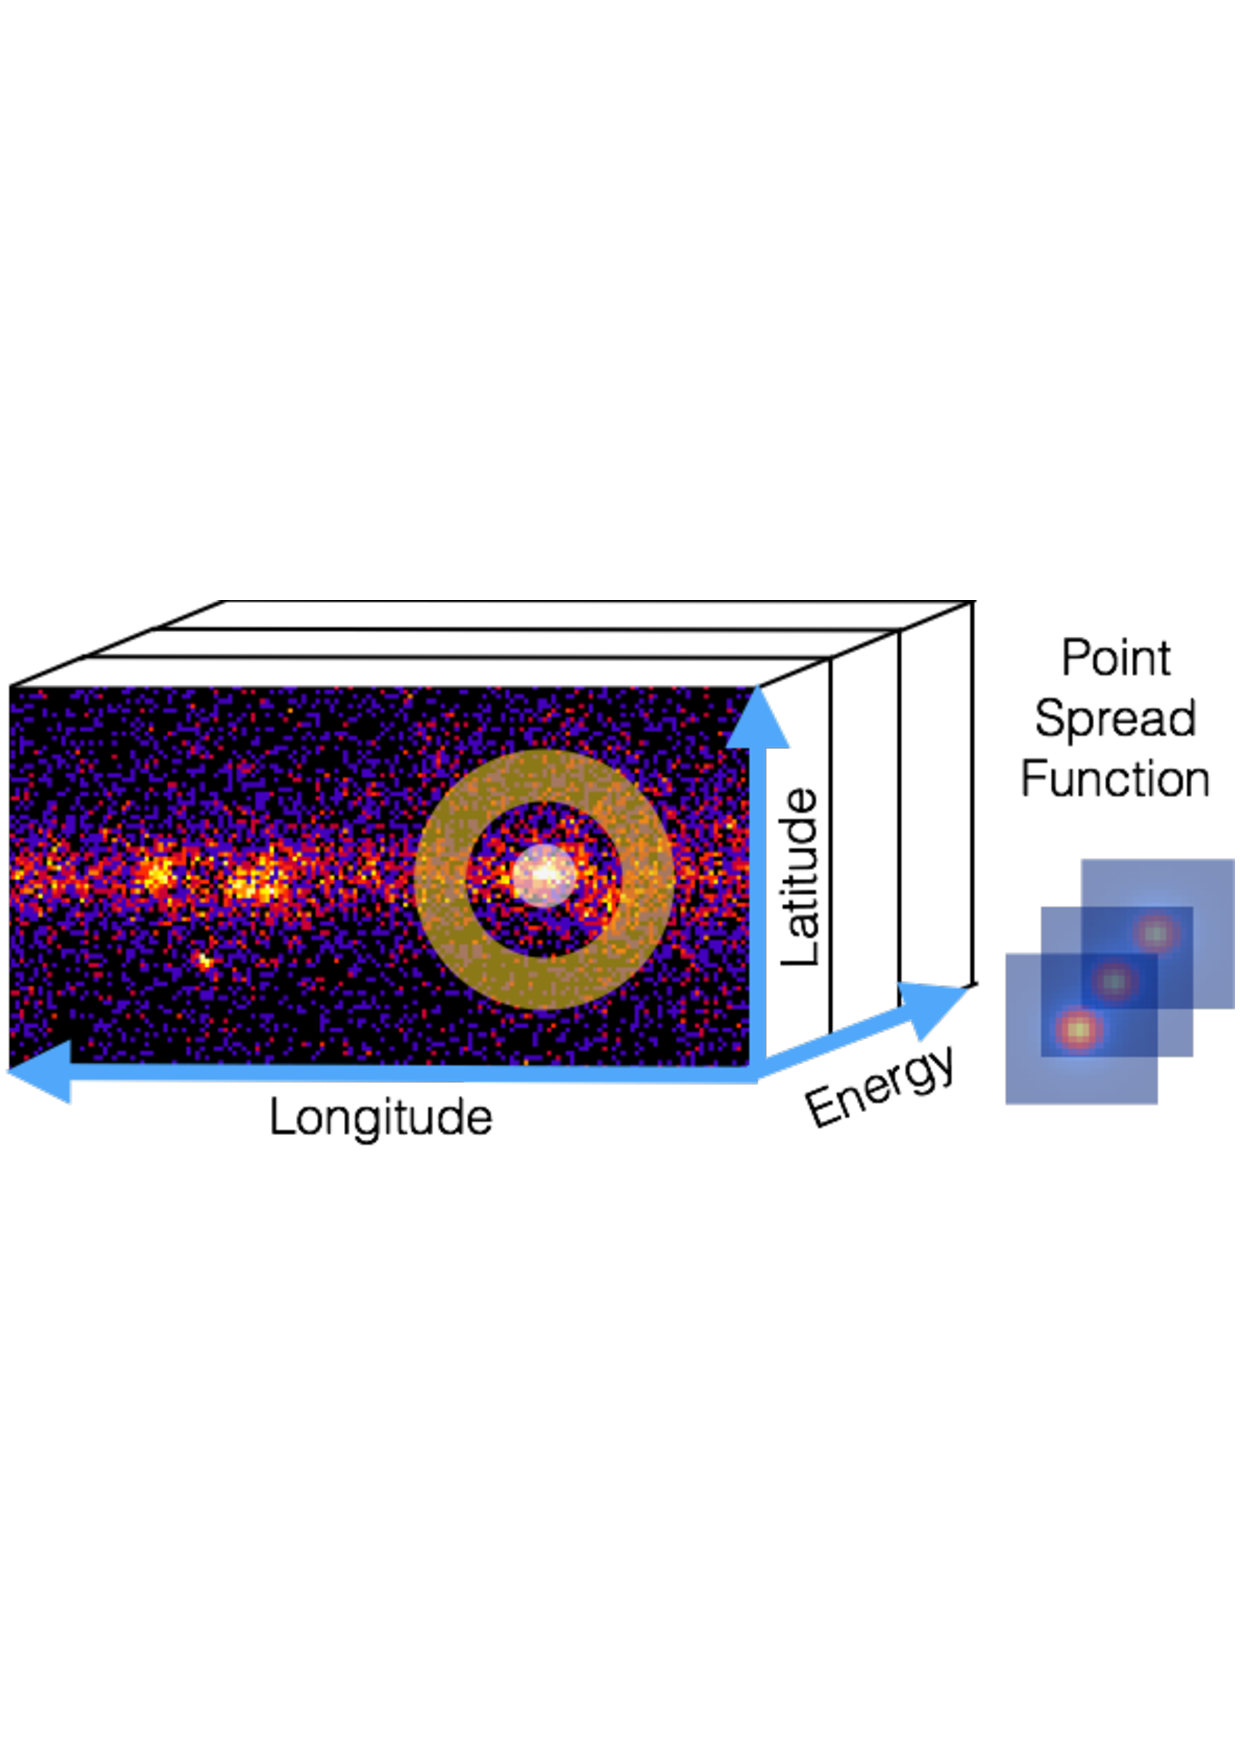
\includegraphics[width=0.8\textwidth]{figures/gammapy-cube-analysis}
\caption{
Gammapy data model illustration. Binned analysis of lon-lat-energy cube data is
supported via joint likelihood analysis of one image per energy bin.
On-off-region based spectral analysis is supported as well.
}
\label{fig:data-model}
\end{figure*}



\subsection{CTA simulation}
\label{sec:apps:cta}

CTA application example.
3D simulate and fit using public prod3 IRFs.
Diffuse emission + maybe a shell -> image and spectrum come out.

\subsection{HESS}
\label{sec:apps:hess}

In September 2018 the HESS collaboration released a small subset of
Gamma-ray data.

Maybe HESS Light curve using PKS flare from HESS
\subsection{Fermi}
\label{sec:apps:fermi}

Fermi: Galactic center, as in our notebook, same region as CTA.

\section{Gammapy project}
\label{sec:project}

Infrastructure etc.

\subsection{Development, testing}

-Github, pytest, CI, PIGs?

\subsection{Documentation}

- Notebooks

\subsection{Software distribution and user support}

- Pip, conda, versions, gammapy download

\subsection{Community}

TODO: Figure: Screenshot of Jupyter notebook or docs with notebook, could show the interactive maps view
\begin{verbatim}
m = Map.read(“diffuse.fits”)
m.plot_interactive()        
\end{verbatim}

\section{Summary and Outlook}
\label{sec:so}


\todo{Axel and Regis write this...}

Summary what we have in v0.9 and presented in this paper.

Roadmap to v1.0, about half a page.

Short conclusion: Gammapy has potential to be the Python package for gamma-ray astronomy.


Prospects for HAWC / SWGO? Or speak in general about water Cherenkov observatories...
\begin{acknowledgements}

We would like to thank the \texttt{Numpy}, \texttt{Scipy}, \texttt{IPython} and
\texttt{Matplotlib} communities for providing their packages which are invaluable
to the development of Astropy. We thank the GitHub team for providing us with
an excellent free development platform. We also are grateful to Read the Docs
(\ReadthedocsUrl), and Travis
(\TravisUrl) for providing free documentation
hosting and testing respectively. Finally, we would like to thank all the
Gammapy users that have provided feedback and submitted bug reports.    
    
TODO: copy over stuff from \url{http://docs.gammapy.org/en/latest/about.html#thanks}.

\end{acknowledgements}


% Back matter
\bibliographystyle{aa}
\bibliography{gammapy-paper.bib}

\end{document}
